\subsection{Badanie wielomianów posiadających wyłącznie pierwiastki rzeczywiste}

\subsubsection{Wielomian o pierwiastkach całkowitych}

Na początku zastanówmy się, jak sprawić, by liczba elementów ciągu Sturma była jak największa. Pozwoli to nam, na zmaksymalizowanie liczby operacji na wielomianach danego stopnia. Aby uzyskać taki wielomian, najłatwiej jest zapewnić, by miał on liczbę pierwiastków rzeczywistych równą lub zbliżoną do jego stopnia. Jak wiemy, liczba ta jest równa różnicy liczby zmian ciągu Sturma w obu przedziałach, a jej wartość jest ograniczona przez liczbę wyrazów tego ciagu. Wynika z tego, że liczba elementów ciagu Sturma jest zawsze większa od liczby pierwiastków rzeczywistych.

Teraz zastanówmy się, jak skonstruować wielomian, który zawiera liczbę różnych pierwiastków rzeczywistych równą jego stopniowi. Intuicyjne utworzenie wielomianu, podając jego kolejne współczynniki jest niemożliwe dla wysokich stopni.

Rozwiązaniem jest więc przedstawienie go w postaci czynników, wskazując jego kolejne pierwiastki. Przykładowo wielomianowi W, o stopniu $k$, możemy przypisać pierwiastki, będące kolejnymi dodatnimi liczbami całkowitymi, ustalając jego wartość jako: \\ $W(x)=(x-1)*(x-2)*(x-3)*...*(x-(k-2))*(x-(k-1))*(x-k)$, gdzie $k$ jest stopniem wielomianu.

Przetestujemy więc wielomiany powyższej postaci. Z powodu ograniczeń czasowych zdecydowałem się w tym teście na badanie wielomianów niższych stopni, niż w pozostałych przypadkach. Zapoznajmy się z rezultatami opisanego eksperymentu.

\begin{table}[H]
	\begin{tabular}{ |p{4cm}|p{2.75cm}|p{2.75cm}|p{3.5cm}|} 
		\hline
		Testowany wielomian & Czas dla PolynomialMap [s] & Czas dla PolynomialVector [s] & Współczynnik czasów \\
		\hline
		$W(x) = x-1$ & 0.003 & 0.003 & 1 \\
		$W(x) = (x-1)(x-2)$ & 0.007 & 0.008 & 1.143 \\
		$W(x) = (x-1)(x-2)(x-3)(x-4)$ & 0.032 & 0.032 & 1 \\
		$W(x) = (x-1)(x-2)*...*(x-7)(x-8)$ & 0.229 & 0.228 & 0.996 \\
		$W(x) = (x-1)(x-2)*...*(x-15)(x-16)$ & 2.404 & 2.391 & 0.995 \\
		$W(x) = (x-1)(x-2)*...*(x-31)(x-32)$ & 29.822 & 29.725 & 0.997 \\
		\hline
	\end{tabular}
	\caption{Porównanie czasów znajdowania pierwiastków dla wielomianów zawierających kolejne pierwiastki całkowite}
\end{table}

Widzimy, że podobnie jak w przypadku wielomianów gęstych zmierzone czasy działania są niemal identyczne dla obu struktur. Jednocześnie trzeba zauwazyć, że duża liczba pierwiastków rzeczywistych wpływa na liczbę elementów ciągu Sturma. Powoduje to mnogość koniecznych do przeprowadzenia operacji na wielomianach, co bezpośrednio przekłada się czas znajdowania pierwiastków w tym przypadku.

\begin{figure}[H]
	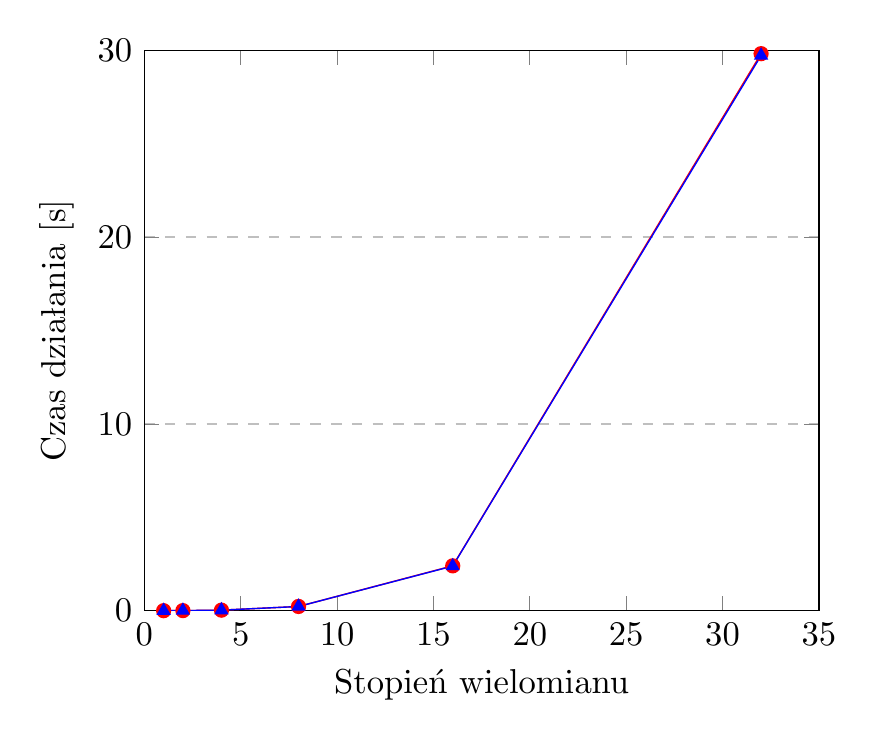
\begin{tikzpicture}[scale=1.25]
	\begin{axis}[
	xlabel={Stopień wielomianu},
	ylabel={Czas działania [s]},
	xmin=0,xmax=35,
	ymin=0,ymax=30,
	ymajorgrids=true,grid style=dashed
	]
	
	\addplot[color=red,mark=*]
	coordinates {
		(1, 0.003)
		(2, 0.007)
		(4, 0.032)
		(8, 0.229)
		(16, 2.404)
		(32, 29.822)
	};
	
	\addplot[color=blue,mark=triangle*]
	coordinates {
		(1, 0.003)
		(2, 0.008)
		(4, 0.032)
		(8, 0.228)
		(16, 2.391)
		(32, 29.725)	
	};
	\end{axis}
	\end{tikzpicture}
	\caption{Czas znajdowania pierwiastków dla wielomianów zawierających kolejne pierwiastki całkowite}
\end{figure}

Obserwując powyższy wykres trzeba zauwazyć wielkie przełożenie stopnia wielomianu na czas działania algorytmu. Wraz z podwojeniem się stopnia testowanego wielomianu widzimy ponad dziesięciokrotny wzrost czasu działania. Tempo wzrostu powyższej funkcji przekracza wzrost sześcienny. Oznacza to, że w przypadku tej klasy wielomianów, której pierwiastkami są kolejne liczby całkowite, mówimy o złożoności wielomianowej.

Niewątpliwy wpływ na wysokie tempo wzrostu ma także wartość kolejnych pierwiastków, która wzrasta wraz ze stopniem wielomianu. Powoduje to, że jesteśmy zmuszeni wykonywać działania na coraz większy liczbach całkowitych. Niektóre z nich posiadają znacznie więcej niż $100$ cyfr, co pomimo użycia biblioteki mpir musi mieć znaczący wpływ na czas wykonywania operacji na liczbach.

\subsubsection{Wielomiany o pierwiastkach wymiernych}

Zachowanie wielomianów może być inne, jeżeli pierwiastki będą się znajdować blisko siebie. By zapewnić im dostatecznie bliskie sąsiedztwo, nie wystarczy by było one liczbami całkowitymi, ale potrzeba by były to liczby wymierne. Podobnie jak w poprzednim przypadku przeprowadzone testy będą zakładały maksymalny stopień wielomianu równy $32$. Dobierzmy odległość pomiedzy pierwiastkami tak, by zapewnić, że odległość między dowolnymi z nich była mniejsza od $1$. Ustalmy, więc ostęp pomiędzy kolejnymi z nich na wartość $0.01.$

Według powyższych założeń testowany wielomian przyjmie następującą wartość: \\ $W(x)=(x-1.01)*(x-1.02)*(x-1.03)*...*(x-(1+\frac{k-2}{100}))*(x-(1+\frac{k-1}{100}))*(x-(1+\frac{k}{100}))$, gdzie $k$ jest stopniem wielomianu.

Zapoznajmy się z wynikami, by sprawdzić, jak uzyskane wyniki różnią się od wcześniejszego przypadku, w którym pierwiastkami były kolejne liczby naturalne.

\begin{table}[H]
	\begin{tabular}{ |p{4cm}|p{2.75cm}|p{2.75cm}|p{3.5cm}|} 
		\hline
		Testowany wielomian & Czas dla PolynomialMap [s] & Czas dla PolynomialVector [s] & Współczynnik czasów \\
		\hline
		$W(x) = x-0.01$ & 0.003 & 0.003 & 1 \\
		$W(x) = (x-0.01)(x-0.02)$ & 0.008 & 0.008 & 1 \\
		$W(x) = (x-0.01)(x-0.02)(x-0.03)(x-0.04)$ & 0.033 & 0.033 & 1 \\
		$W(x) = (x-0.01)(x-0.02)*...*(x-0.07)(x-0.08)$ & 0.229 & 0.228 & 1 \\
		$W(x) = (x-0.01)(x-0.02)*...*(x-0.15)(x-0.16)$ & 9.275 & 9.291 & 1.002 \\
		$W(x) = (x-0.01)(x-0.02)*...*(x-0.31)(x-0.32)$ & 1226.351 & 1226.333 & 1 \\
		\hline
	\end{tabular}
	\caption{Porównanie czasów znajdowania pierwiastków dla wielomianów zawierających pierwiastki wymierne różniące się o $0.01$}
\end{table}

\begin{figure}[H]
	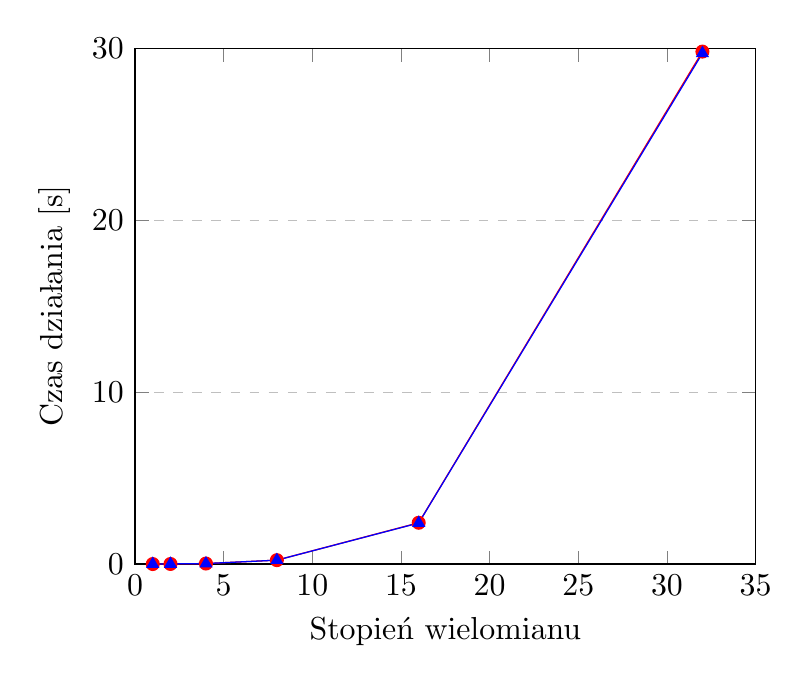
\begin{tikzpicture}[scale=1.15]
	\begin{axis}[
	xlabel={Stopień wielomianu},
	ylabel={Czas działania [s]},
	xmin=0,xmax=35,
	ymin=0,ymax=30,
	ymajorgrids=true,grid style=dashed
	]
	
	\addplot[color=red,mark=*]
	coordinates {
		(1, 0.003)
		(2, 0.007)
		(4, 0.032)
		(8, 0.229)
		(16, 2.404)
		(32, 29.822)
	};
	
	\addplot[color=blue,mark=triangle*]
	coordinates {
		(1, 0.003)
		(2, 0.008)
		(4, 0.032)
		(8, 0.228)
		(16, 2.391)
		(32, 29.725)	
	};
	\end{axis}
	\end{tikzpicture}
	\caption{Czas znajdowania pierwiastków dla wielomianów zawierających pierwiastki wymierne różniące się o $0.01$}
\end{figure}

Podobnie jak dla wszystkich innych wielomianów gęstych także w tym przypadku w wyniku porównania struktur otrzymujemy bliźniacze rezultaty. Jednocześnie należy zwrócić uwagę, że wartość pierwiastków wielomianu ma bardzo duże przełożenie na czas ich znajdowania. Widzimy, że w przypadku blisko siebie położonych pierwiastków o niewielkich wartościach zmiennoprzecinkowych czas działania algorytmu jest kilkadziesiąt razy większy niż dla kolejnych liczb naturalnych. Kluczowe wydają się w tym przypadku dwa aspekty. Pierwszym z nich jest konieczność pracy na liczbach niecałkowitych, co powoduje znaczną komplikację działań. Drugim z nich może być wspomniana wcześniej bliskość kolejnych pierwiastków, która powoduje, że pomimo znacznego zawężania przedziału wyszukiwań, w danym zakresie wciąż może znajdować się w nim więcej niż jeden pierwiastek.
